\documentclass[12pt]{article}
\usepackage[margin=1in]{geometry}
\usepackage{graphicx}
\usepackage{caption}
\usepackage{subcaption}
\usepackage{amsmath}
\usepackage{hyperref}
\usepackage{float}
\usepackage{cite}
\usepackage{booktabs}
\usepackage{enumitem}

\title{Technical Report}
\author{Priyangika Pitawala}
\date{April 16, 2025}   

\begin{document}

\maketitle

The code repository can be accessed at \url{https://github.com/PriyaPitawala/cmse802_project}.

\section*{Project Title}
Image Analysis and Percent Crystallinity Quantification

\section{Introduction}

\subsection{Project Overview}
This project involves creating a Python-based tool that processes polarized optical microscope (POM) images of a semicrystalline
thiol-ene photopolymer system suited for vat photopolymerization (VP), and analyzes the percent crystallinity. It will also attempt to 
find a correlation between the crystallinity features and the VP processing parameters such as light intensity,
layer thickness, photoabsorber concentration.

\subsection{Objectives}
\begin{itemize}[noitemsep]
    \item To preprocess the POM images to enhance the contrast between crystalline and amorphous regions, and to reduce noise.
    \item To define the features that characterize crystallinity and develop an algorithm to distinguish between crystalline and amorphous regions.
    \item To calculate the percent crystallinity of each image and aggregate the results of multiple images using statistical methods.
    \item To analyze the relationships between the percent crystallinity and the polymer processing parameters
    \item To use data visualization tools to display the results.
    
\end{itemize}

\subsection{Significance of the Problem}
Semicrystalline morphology directly influences the thermal and mechanical performance of photopolymers used in VP. 
Accurate analysis is crucial for optimizing these materials.

\subsection{Scope and Limitations}
The project focuses on segmenting spherulites and Maltese cross from grayscale POM images of semicrystalline polymers, 
assuming uniform lighting and minimal image noise. Extension to other microscopy and materials types is outside scope.

\section{Project Implementation}

\subsection{Architecture and Component Overview}
The tool is organized into modular Python scripts:
\begin{itemize}[noitemsep]
    \item data\_loading/ -- loads raw POM images and metadata
    \item preprocessing/ -- preprocesses images to enhance contrast and reduce noise
    \item segmentation/ -- segments the images using edge-based techniques and watershed algorithm
    \item feature\_extraction/ -- extracts crystallinity features
    \item crystallinity\_quantification/ -- calculates percent crystallinity and size distribution
    \item regression/ -- performs regression analysis to find correlations between crystallinity and processing parameters
    \item visualization/ -- generates plots and overlays
\end{itemize}

\subsection{Implementation Status}
Most pipeline components are functional. Remaining modelling tasks include refining gradient-based splitting of merged spherulites and 
optimizing the preprocessing step to reduce oversegmentation. 

Forming correlations between crystallinity and processing parameters was completed, however, including material properties will require
 additional data collection. Furthermore, certain processing parameters produced images with significant noise, making segmentation 
 difficult. Handling these cases will require further refinement of the data collection and preprocessing steps.

\subsection{Key Algorithms and Methods Used}
\begin{itemize}[noitemsep]
    \item Grayscale conversion for color image processing
    \item Adaptive histogram equalization (CLAHE) for contrast enhancement
    \item Noise reduction using grain size filtering for foreground and background separation
    \item Further noise reduction using Gaussian blur and thresholding before watershed segmentation
    \item Initial segmentation using edge-based techniques (Canny edge detection)
    \item Computation of markers for watershed segmentation
    \item Watershed algorithm for separating merged spherulites
    \item Quantitative feature extraction for crystallinity metrics
    \item Percent crystallinity calculation using size distribution of segmented regions
    \item Weighted averaging of crystallinity features grouped by processing parameters
    \item Visualization of crystallinity features against processing parameters to find correlations
\end{itemize}

\subsection{Technical Challenges and Solutions}
Noisy edges and merged spherulites pose a challenge. Refinement of the segmentation is underway with the following strategies:
\begin{enumerate}[noitemsep]
    \item Increase the threshold for size filtering to remove small noise particles.
    \item Use gap closing and dilation to fill gaps in the edges and separate merged spherulites.
    \item Implement a hybrid edge-watershed segmentation approach to combine edge-based and watershed techniques.
\end{enumerate}

\subsection{Changes from HW2 Plan}
Rather than structure-property correlations, the focus shifted to processing-structure correlations.

This change was made to better align with the available data and to make the project more manageable within the given timeline.
Future work will include exploring the relationship between crystallinity and material properties, after difficulites with 
segmenting complicated images are resolved.

\section{Technical Optimization}

\subsection{Performance Bottlenecks Identified}
Difficulty in preprocessing images in batch mode due to variations in noise levels. Thus, the preprocessing step must be 
closely tailored to each image. This can be time-consuming and inefficient, especially when processing large datasets.

\subsection{Optimization Techniques Implemented}
Vectorized NumPy operations and investigating multiple segmentation techniques.

\subsection{Quantitative Performance Improvements}
Creating a foreground mask based on expert knowledge of the images has improved the segmentation accuracy.

Masking removed a significant amount of noise and allowed for more accurate segmentation of the crystalline regions.

\subsection{Error Handling and Robustness Measures}
Input shapes and image channels are validated to check if the input is a valid image. This ensures that the program does not 
crash when given an invalid input. In such cases, a ValueError is raised, and the user is prompted to check the input.

Segmentation steps are modular for fallback. If a segmentation step fails, the program can revert to the previous step and 
try again with different parameters or segmentation techniques.
This allows for flexibility in the segmentation process and ensures that the program can still produce results even if one 
step fails.

\section{Validation and Testing}

\subsection{Validation Methodology}
Manual visual inspection and cross-comparison with annotated samples. This involves overlaying removed noise, segmented regions, and
extracted features on the original image to ensure that the segmentation is accurate and that the features are correctly extracted.

\subsection{Test Cases and Coverage}
Tested across image sets varying in contrast, crystallinity, and lighting. As the samples were prepared under different conditions, 
this was an expected outcome. The images were taken by maintaining similar color histograms. 

Some images are thicker than others, causing multiple spherulite layers to be included in the same image. This increased the level of 
noise. To mitigate this, the segmentation quality was scored to weigh the statistical results. Figure 1 shows an 
example of a raw image with high noise levels. Figure 2 shows the same image after segmentation and feature extraction, where the 
segmentation accuracy is low. In contrast, Figure 3 show a raw image with low noise levels, and Figure 4 shows the same image after 
segmentation and feature extraction, where the segmentation accuracy is high.

\begin{figure}[H]
    \centering
    \includegraphics[width=0.6\textwidth]{figures/S72_1_raw.png}
    \caption{\centering Raw POM image with high level of noise.}
\end{figure}

\begin{figure}[H]
    \centering
    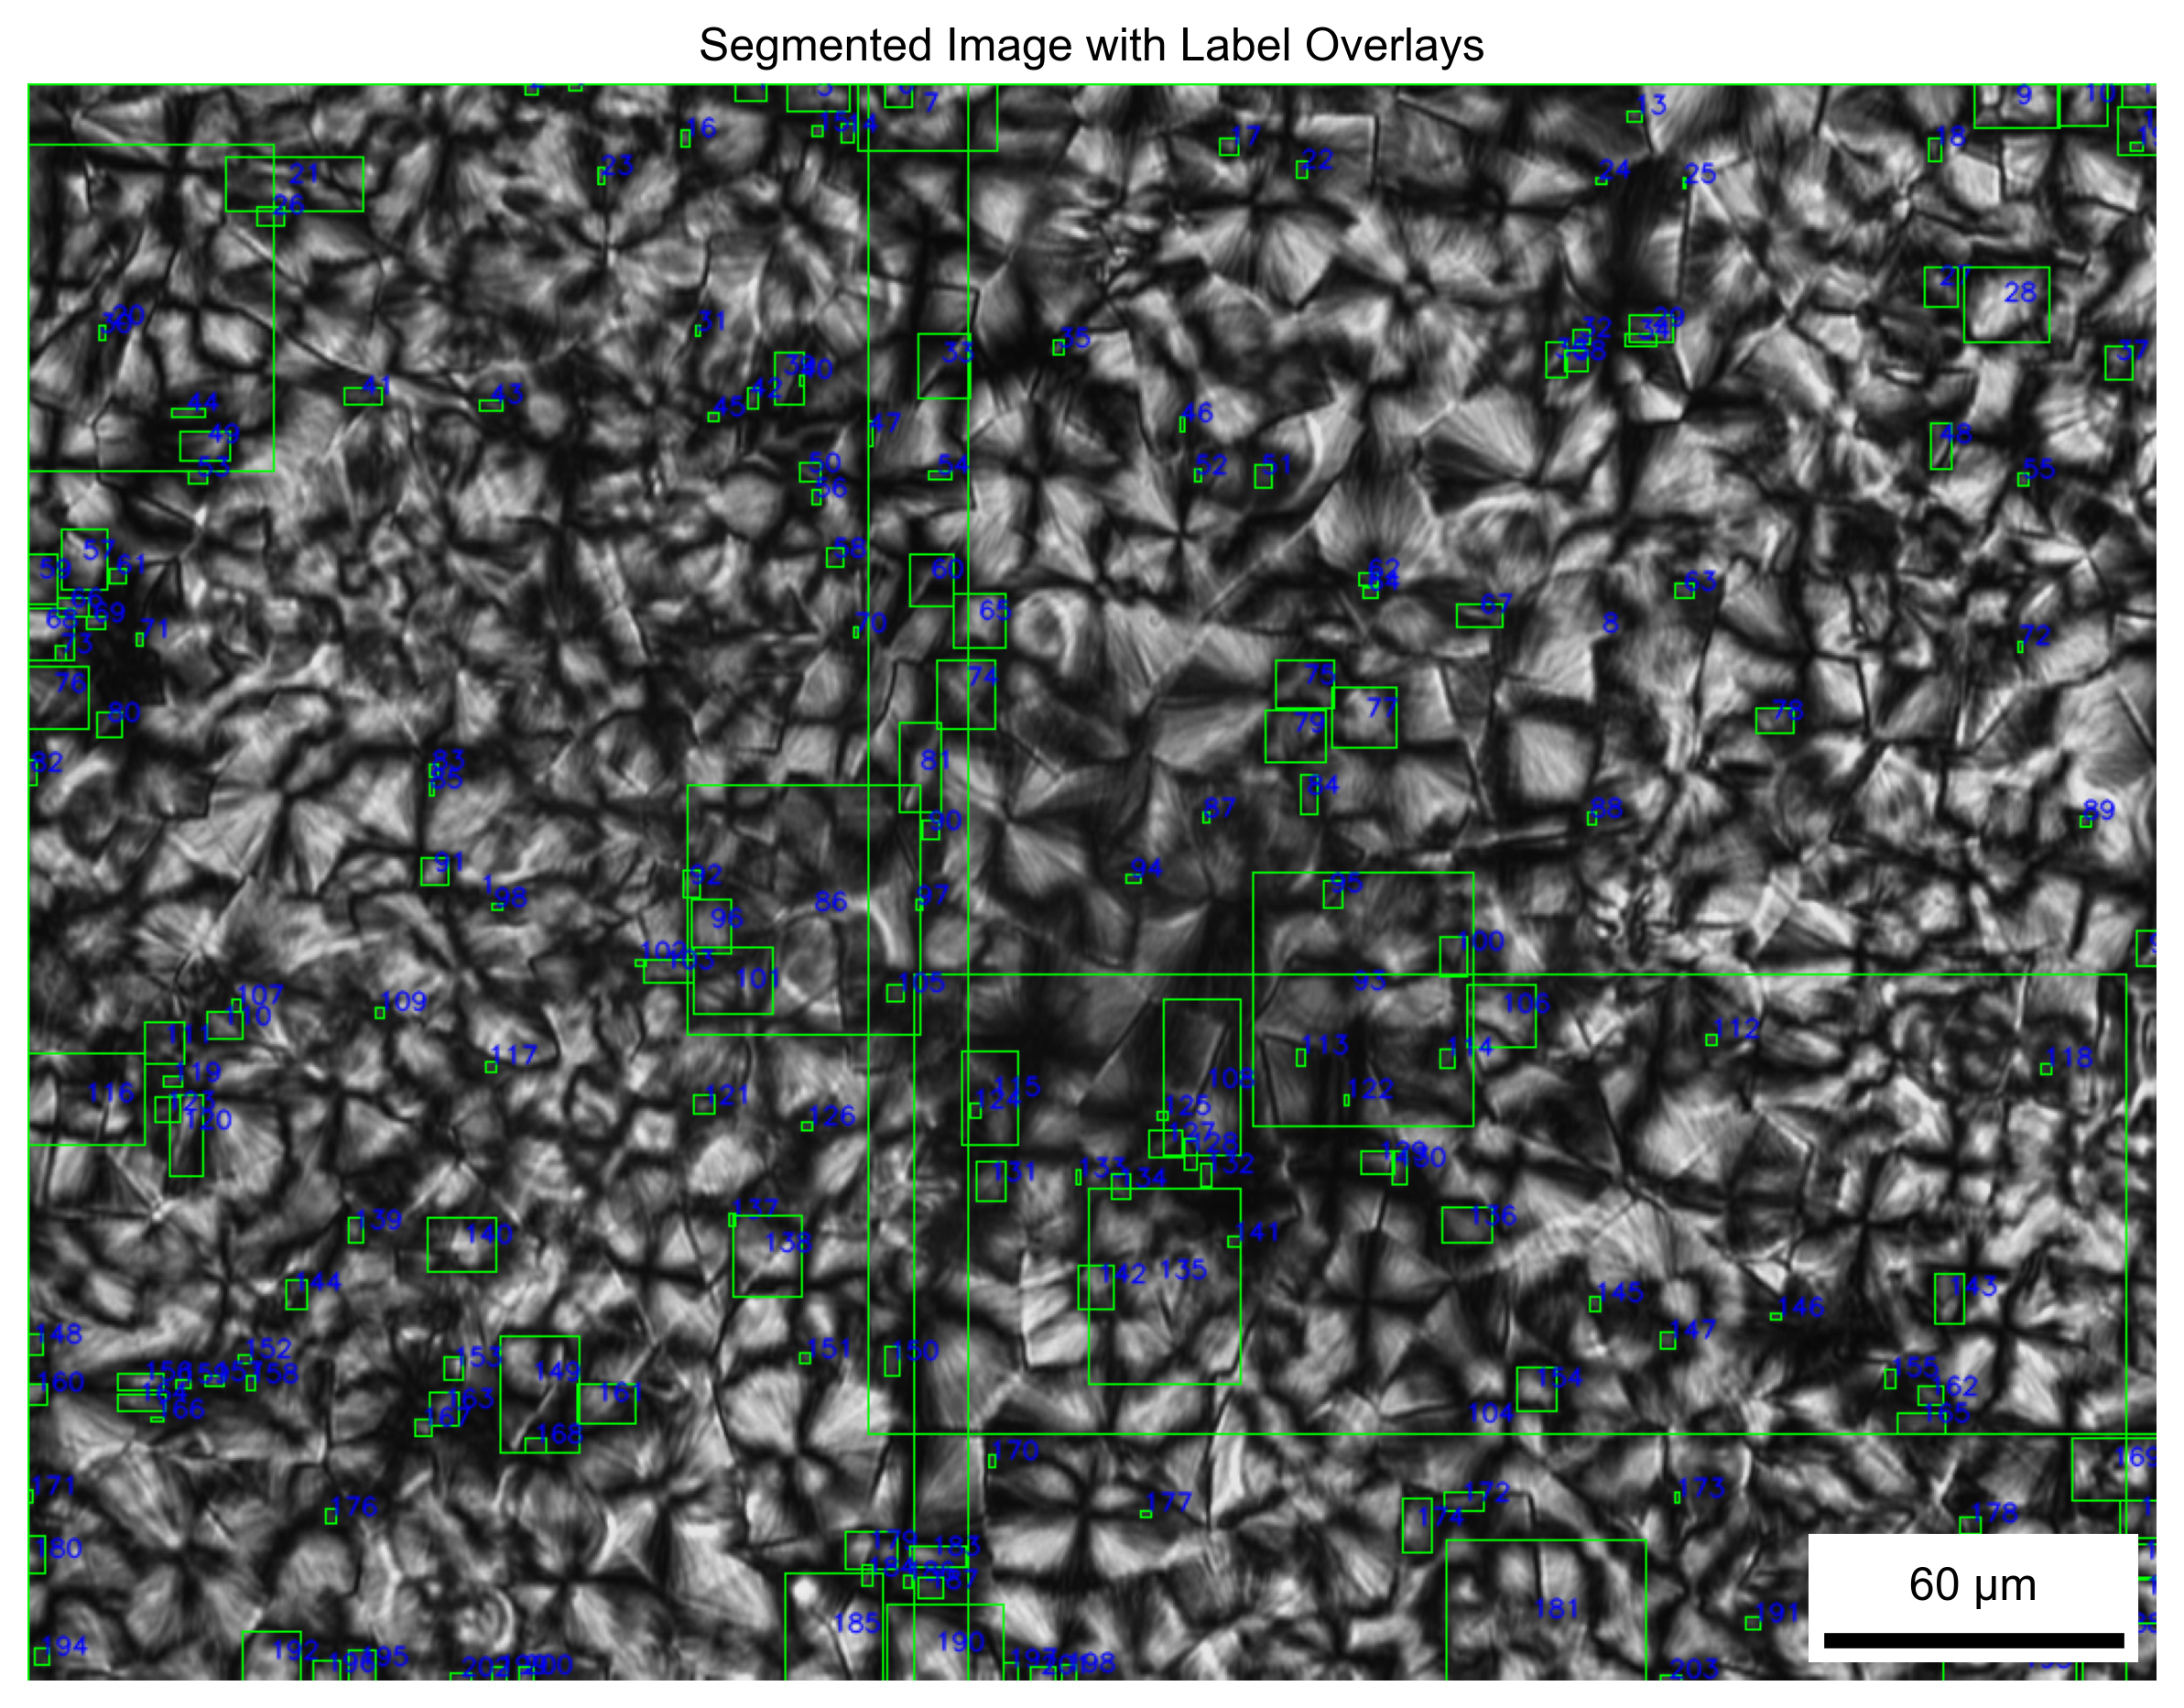
\includegraphics[width=0.6\textwidth]{figures/S72_1_extract.png}
    \caption{\centering Extracted features from Figure 1. Most spherulites remain unidentified, as high noise levels 
    have interefered with the segmentation}
\end{figure}

\begin{figure}[H]
    \centering
    \includegraphics[width=0.6\textwidth]{figures/S58_3_raw.png}
    \caption{\centering Raw POM image with low level of noise.}
\end{figure}

\begin{figure}[H]
    \centering
    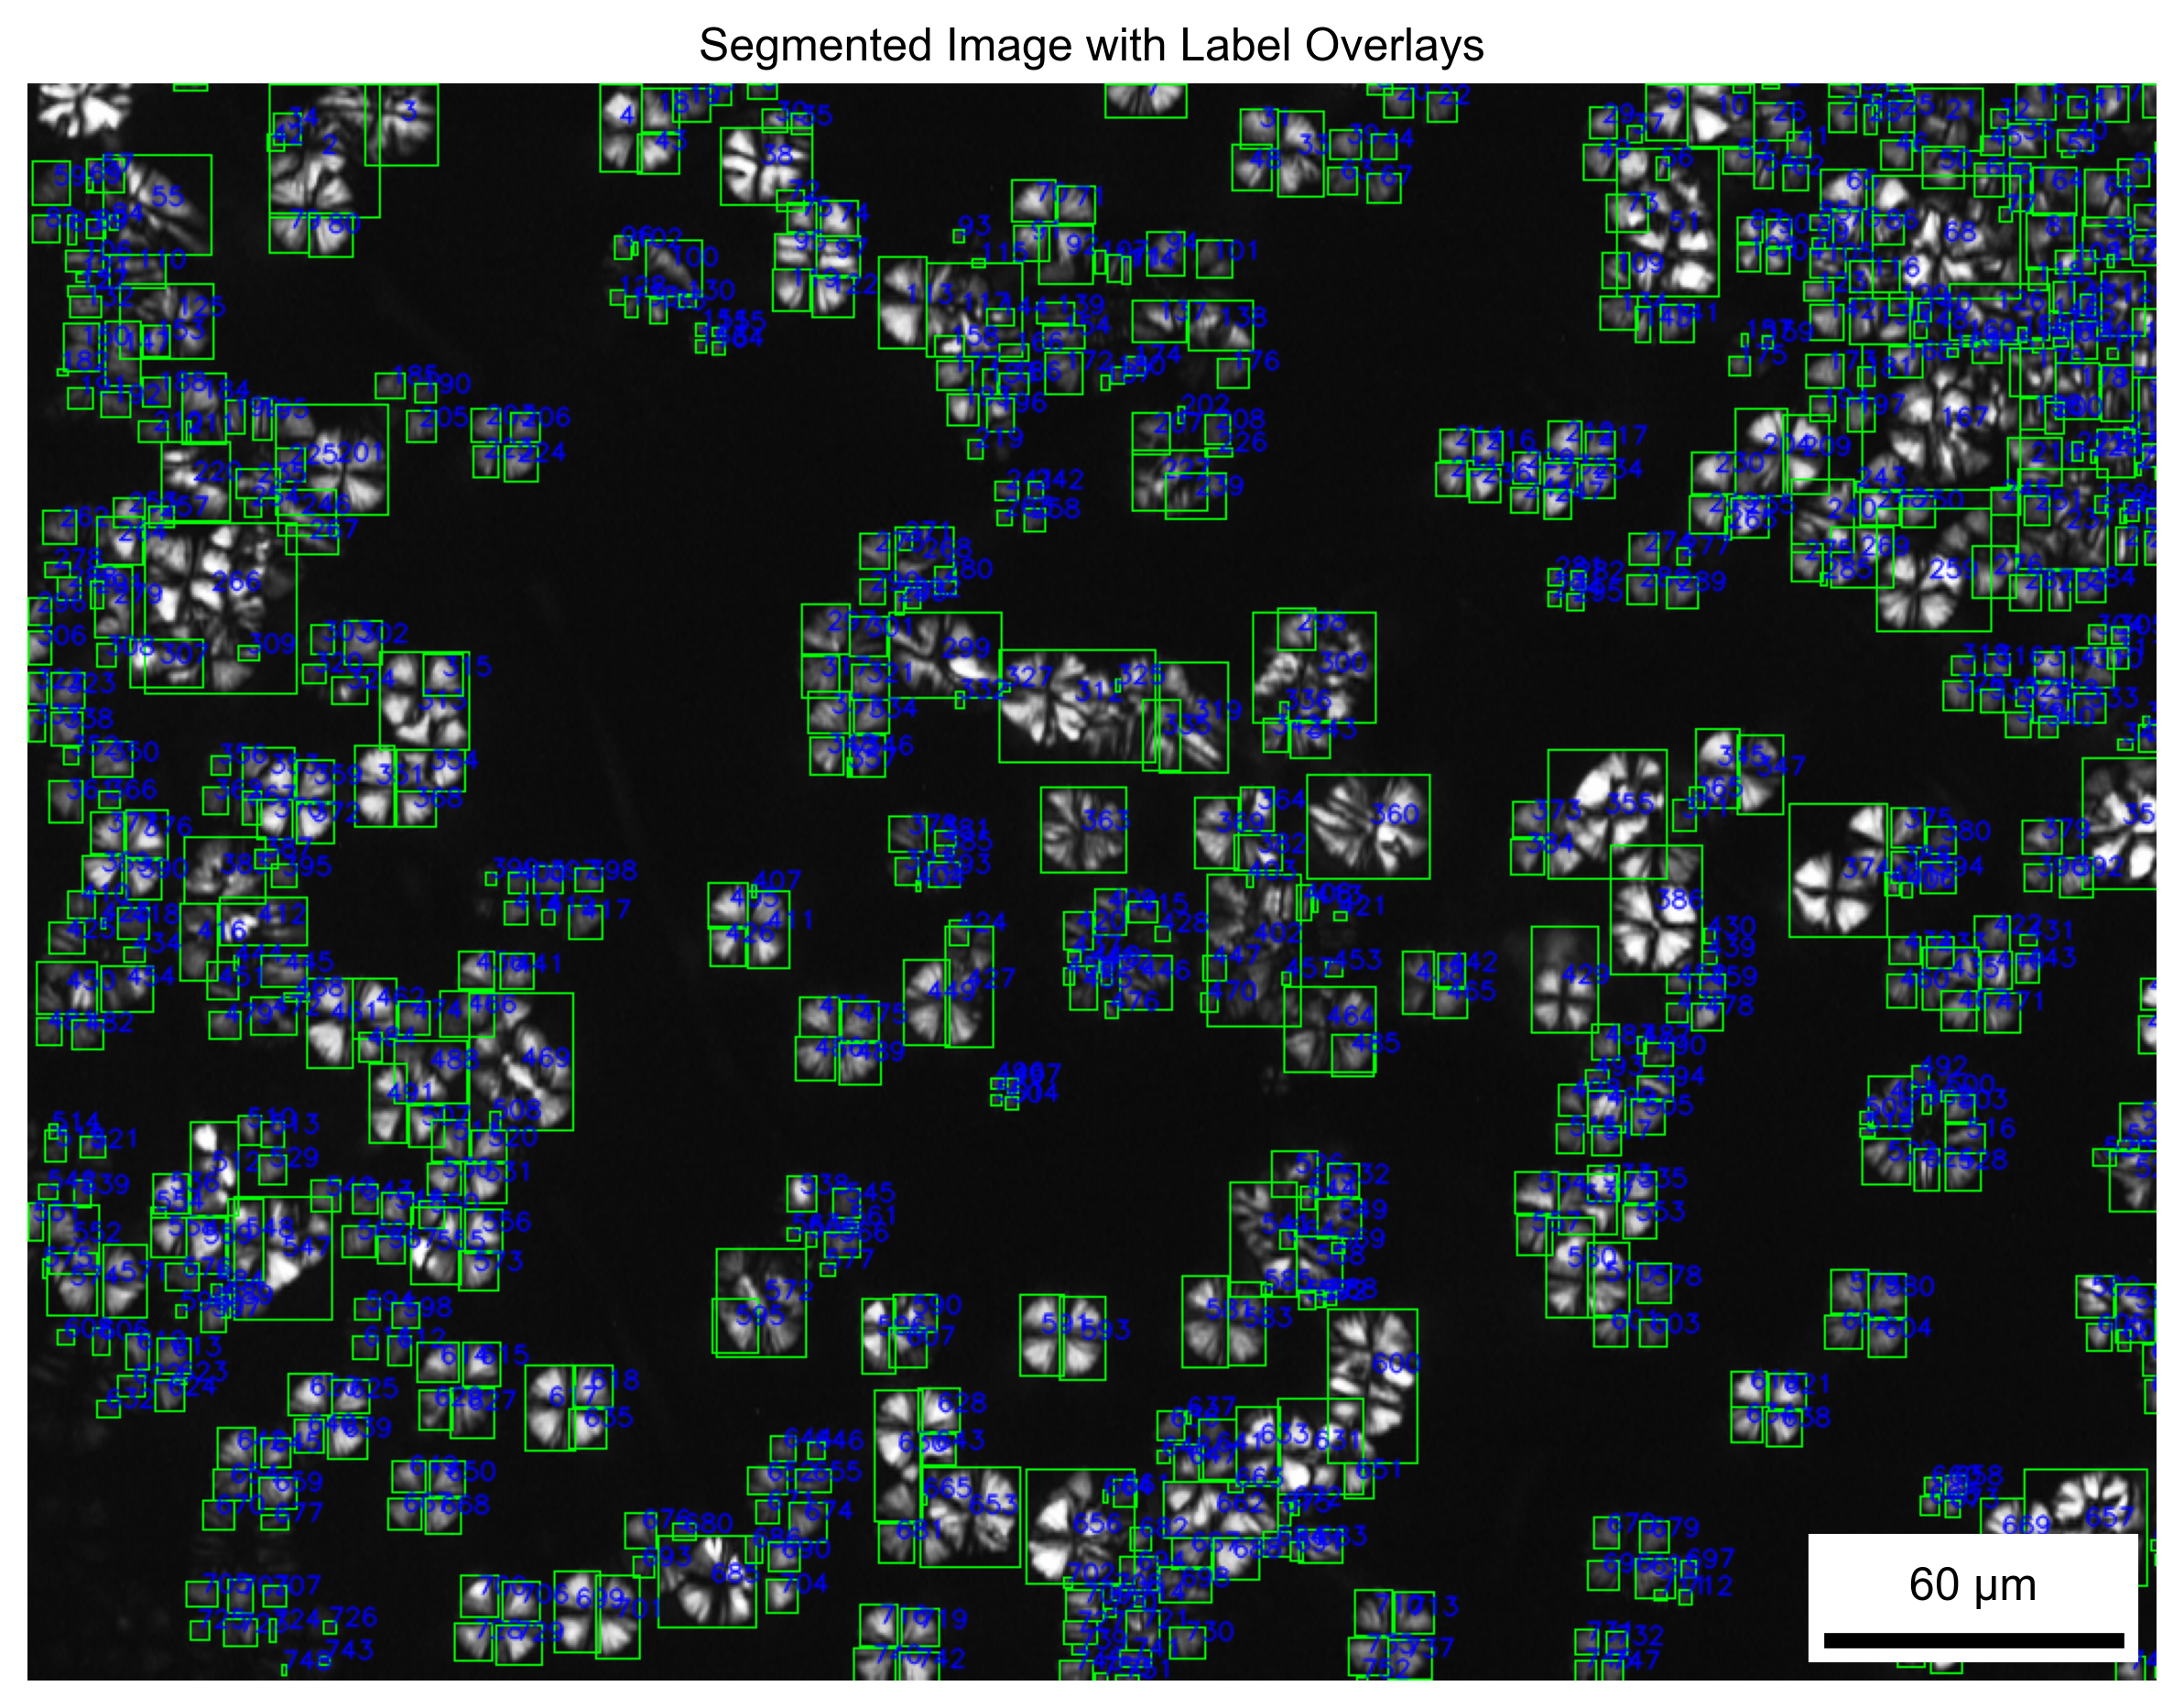
\includegraphics[width=0.6\textwidth]{figures/S58_3_extract.png}
    \caption{\centering Extracted features from Figure 3. Segmentation accuracy is high, as most spherulites are
    identified.}
\end{figure}

\subsection{Quantitative Validation Results}
Results were validated by visual inspection such as in Figures 1-4. 

\subsection{Analysis of Accuracy and Reliability}
Segmentation is reliable for clear boundaries. Undersegmentation may occur in low-contrast regions.

\section{Results and Discussion}

\subsection{Key Findings and Outputs}
Edge-based segmentation performed well on high-contrast images, which correponded to higly amorphous regions.

Low light intensities produced highly crystalline surfaces, with grain boundaries visible in the images. However,
the segmentation was less reliable in these cases, as the spherulites were not clearly defined. Therefore, a hybrid 
approach may be necessary to improve the segmentation accuracy.

Figure 5 shows the general trend of crystallite size dristribution with respect to the processing parameters.

\begin{figure}[H]
    \centering
    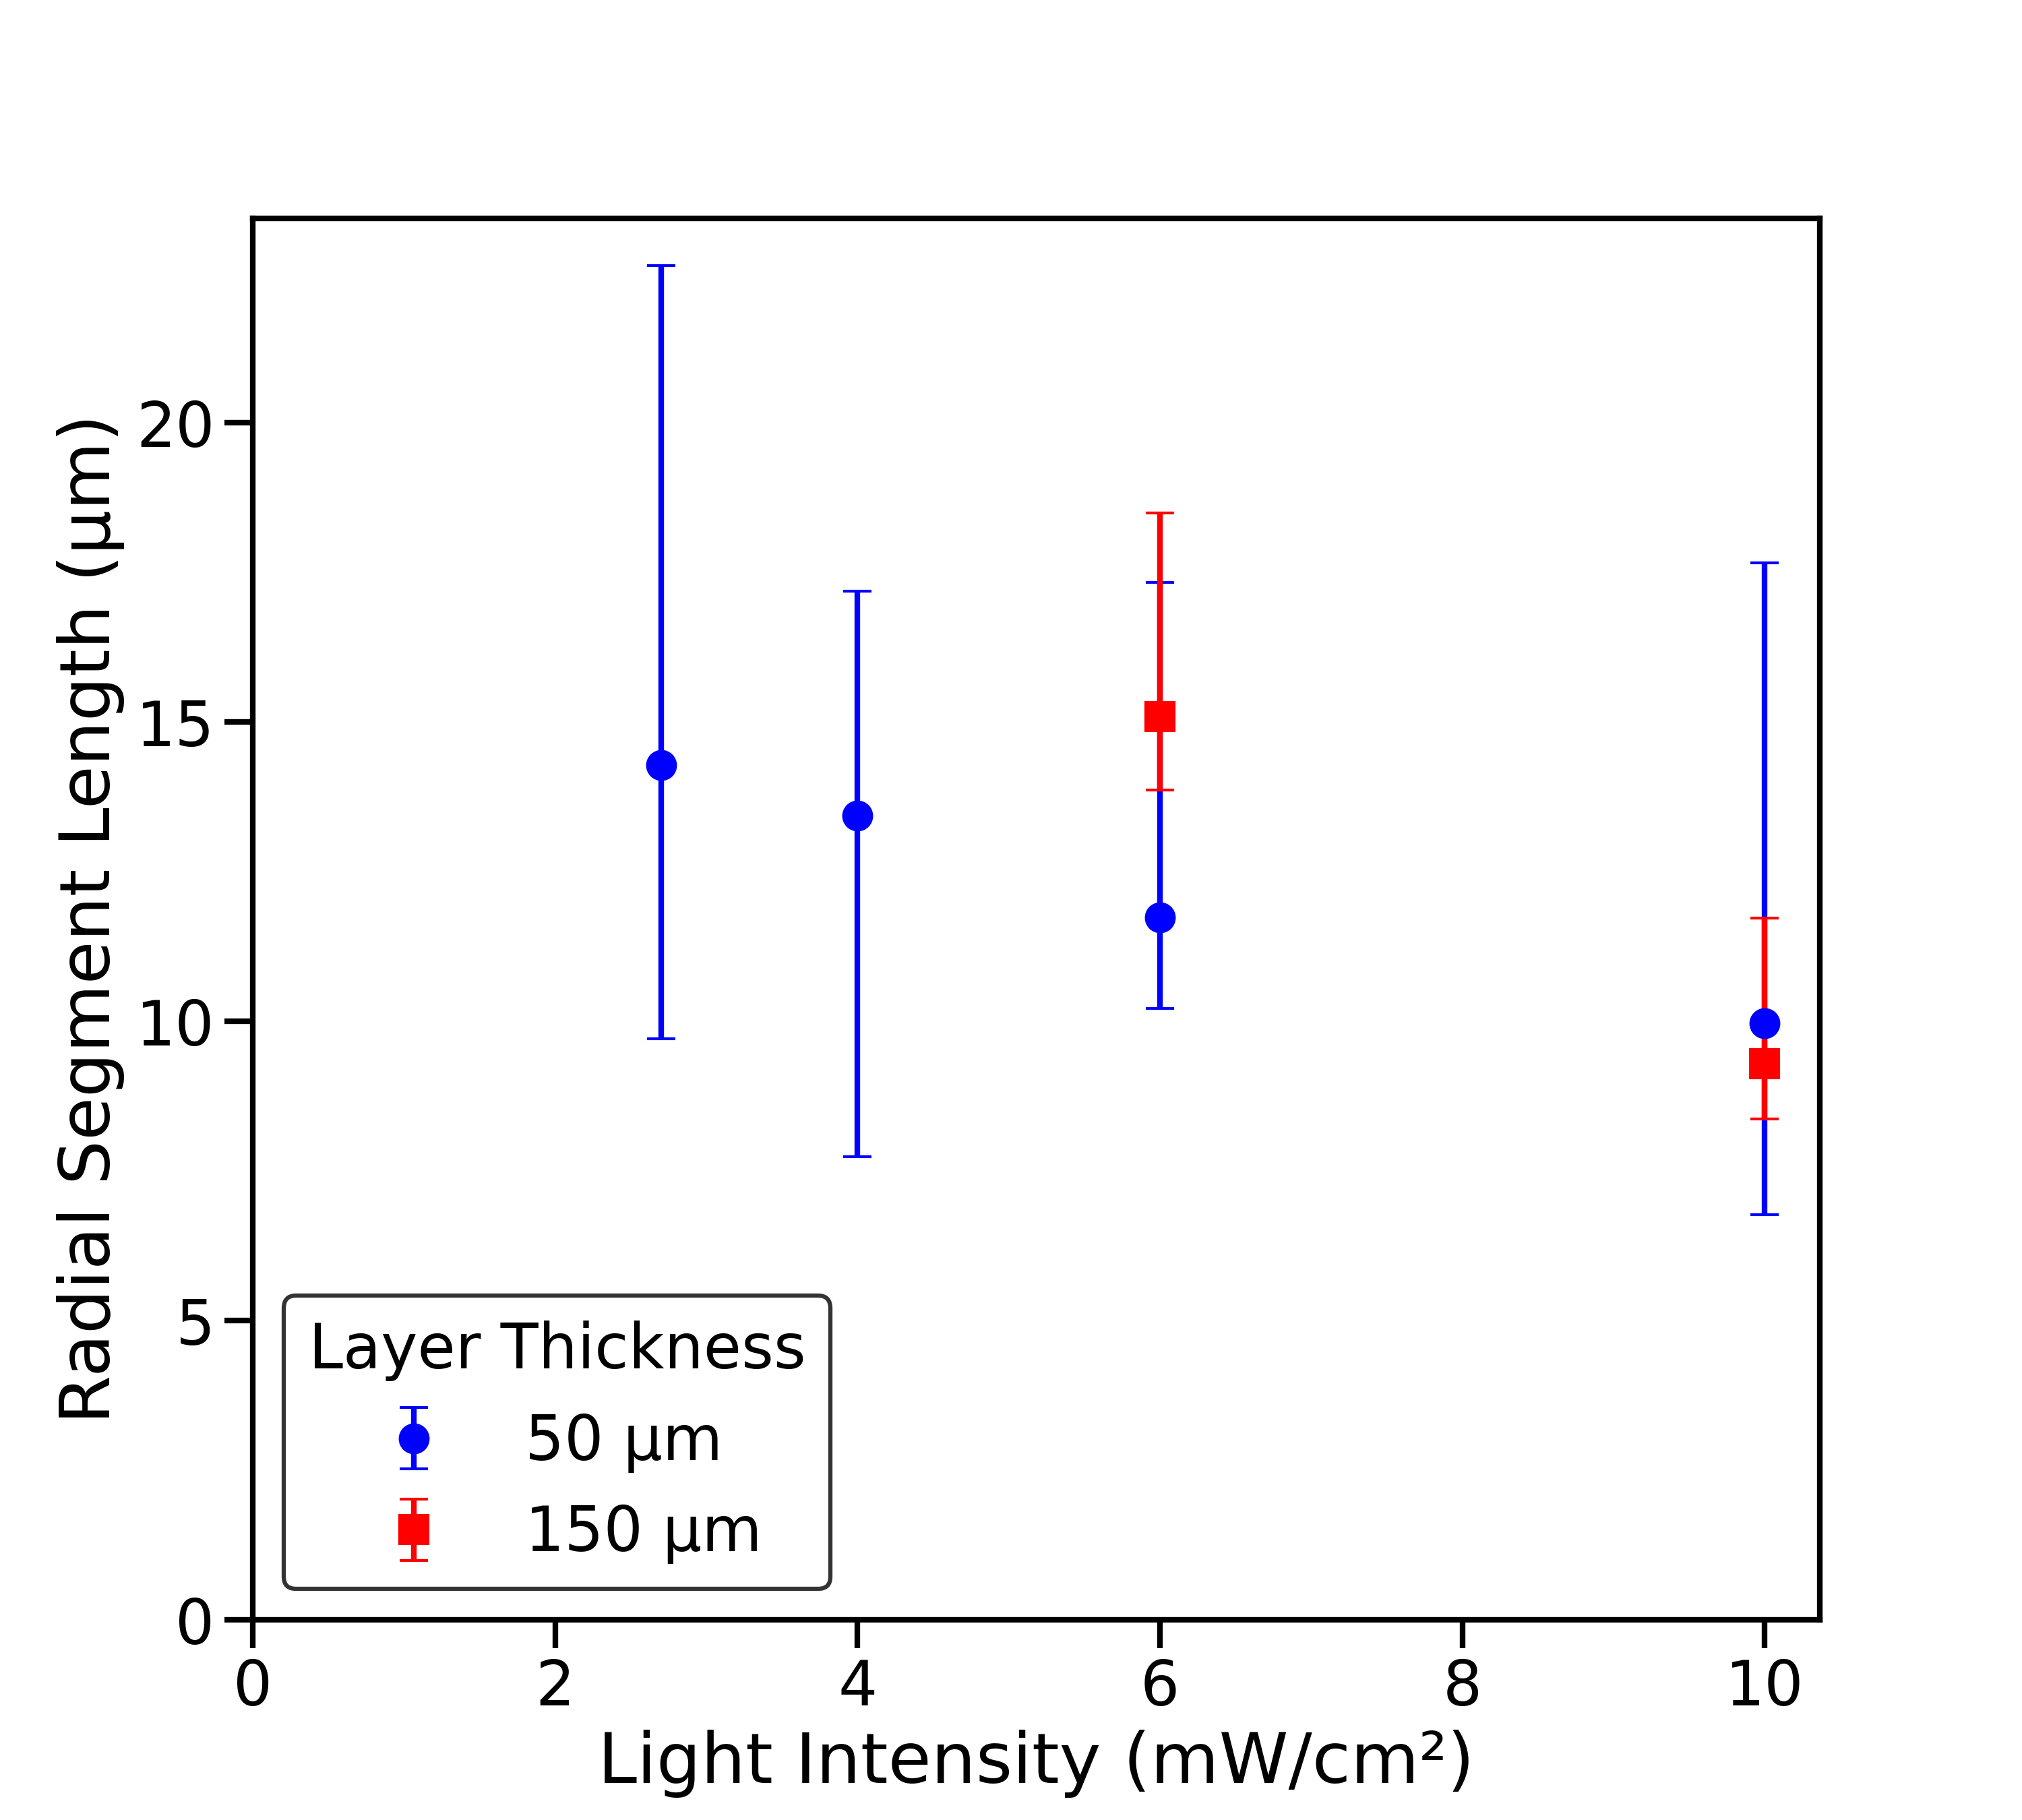
\includegraphics[width=0.6\textwidth]{figures/median_diameter_vs_light_0.1wt.png}
    \caption{\centering Median radial segment length of spherulites as a function of light intensity and layer thickness.
    The data is grouped by photoabsorber concentration of 0.1 wt\%.}
\end{figure}


\subsection{Analysis of Results}
Lower light intensities and thicknesses promote heterogeniety in crystallization. Therefore, the spherulite 
size distribution is wider, as shown in Figure 5. 

Furthermore, due to potential skewing from over- or under-segmentation, the mean spherulite size was not a good
indicator of the crystallinity. The median spherulite size was used instead, as it is less sensitive to outliers.

\subsection{Interpretation in Context of Project Goals}
The model is able to segment and quatify the semicrystalline morphology of the thiol-ene photopolymer system.
The performance was better at certain processing parameters, and while refinement is required for improving
segmentation accuracy, the model is able to produce interpretable metrics.

\subsection{Limitations and Future Improvements}
Segmentation errors persist in thicker samples, due to poor image quality. Future work will include 
better data collection steps, and tuning of the preprocessing parameters to improve the segmentation accuracy.

\section{Conclusion}

\subsection{Summary of Achievements}
An image analysis tool for segmenting and quantifying semicrystalline morphology from POM images was developed.
The model is tunable for different noise levels, with all the preprocessing and segmentation steps modularized for flexibility.
Meaningful correlations were made between crystallinity and processing parameters, and the results were visualized using Matplotlib.

\subsection{Evaluation of Approach}
The image processing pipeline builds up from basic steps such as grayscale conversion and histogram equalization, 
to more complex steps such as watershed segmentation and feature extraction. This approach allowed for a clear understanding
of the segmentation process and the ability to fine-tune each step for better results. Furthermore, it ensured that simpler 
solutions were not overlooked in favor of more complex ones.

\subsection{Next Steps for Completion}
Adjusting preprocessing parameters for better segmentation, and attempting to find a correlation between crystallinity and
 material properties.

\section{References}
\begin{itemize}
    \item Gonzalez, R. C., and Woods, R. E. \textit{Digital Image Processing}, 4th ed., Pearson, 2018.
    \item OpenCV: https://opencv.org/
    \item Scikit-Image: https://scikit-image.org/
    \item NumPy: https://numpy.org/
    \item Matplotlib: https://matplotlib.org/
    \item OpenAI. \textit{ChatGPT}; https://chat.openai.com (accessed April 16, 2025).
\end{itemize}

\end{document}

